% concatenated from Connected.tex
\documentclass[a4paper,12pt]{amsart}

\usepackage{a4wide}
\usepackage{pgf,tikz}
\usepackage{amssymb}
\usepackage{enumerate}
	
\usepackage{amsmath}

\newif\ifdetails
\detailstrue
\newcommand{\DETAIL}[1]%
{\ifdetails\par\fbox{\begin{minipage}{0.9\linewidth}\textit{Detail:}
      #1\end{minipage}}\par\fi}
\newcommand{\TODO}[1]%
{\ifdetails\par\fbox{\begin{minipage}{0.9\linewidth}\textbf{TODO:}
      #1\end{minipage}}\par\fi}


\usepackage{makecell}
\usepackage{relsize}


\usepackage[pagewise,displaymath, mathlines]{lineno}
%\linenumbers


\newtheorem{lemma}{Lemma}
\newtheorem{proposition}[lemma]{Proposition}
\newtheorem{theorem}[lemma]{Theorem}
\newtheorem{corollary}[lemma]{Corollary}
\theoremstyle{remark}
\newtheorem{example}{Example}
\newtheorem{remark}{Remark}
\newtheorem{conjecture}{Conjecture}
\newtheorem{question}{Question}
\newtheorem{definition}[lemma]{Definition}
\newtheorem{problem}{Problem}
\DeclareMathOperator{\N}{N}
\DeclareMathOperator{\diam}{diam}
\DeclareMathOperator{\V}{V}
\DeclareMathOperator{\E}{E}
\DeclareMathOperator{\C}{c}
\DeclareMathOperator{\n}{n}
\usepackage{caption}
\usepackage{subcaption}
%\captionsetup[subfigure]{labelformat=empty}

%\usepackage[below,section]{placeins} % the one below is better for short assignments
\usepackage{float} % provides H as float placement specifier
% extras
\usepackage[pdftex,a4paper,citecolor = blue, colorlinks=true,urlcolor=blue]{hyperref}
\urlstyle{same}

%
\newcommand*{\KeepStyleUnderBrace}[1]{%
  \mathop{%
    \mathchoice
    {\underbrace{\displaystyle#1}}%
    {\underbrace{\textstyle#1}}%
    {\underbrace{\scriptstyle#1}}%
    {\underbrace{\scriptscriptstyle#1}}%
  }\limits
}

\usepackage{mathrsfs}
\usetikzlibrary{arrows}

%\usepackage{mathtools}



\newcommand{\old}[1]{{}}
\newcommand{\mnote}[1]{\marginpar{\raggedright\footnotesize\em#1}}%Marginal Note
%\usepackage[notref,notcite]{showkeys}


\title{Bicyclic graphs with the smallest and largest numbers of connected sets}

\author{Audace A. V. Dossou-Olory}
\thanks{}

\address{Audace A. V. Dossou-Olory \\ Institut National de l'Eau \\ and  Institut de Math\'ematiques et de Sciences Physiques, Dangbo \\ Universit\'e d'Abomey-Calavi, B\'enin \\ \newline \textbf{ORCID} \url{0000-0003-2065-117X}}
\email{audace@aims.ac.za} \email{audace.dossouolory@uac.bj}

\subjclass[2020]{Primary 05C30; secondary 05C35, 05C69, 05C75}
\keywords{bicyclic graphs, connected sets, extremal structures, induced subgraphs}


\begin{document}


\begin{abstract}	
For a graph $G$ with vertex set $V$, let $\N(G)$ denote the number of nonempty subsets of $V$ that induce a connected graph in $G$. In this paper, we focus on determining $\N(G)$ for $G$ in the family $\mathbb{B}_n$ of $n$-vertex bicyclic graphs. We find in $\mathbb{B}_n$ the structures of those graphs that possess the smallest, the largest, as well as the second-largest values of $\N(G)$. Moreover, we compute the extreme values of $\N(G)$ over $ \mathbb{B}_n$.
\end{abstract}

\maketitle

\section{Introduction}\label{Intro:main}


All graphs considered in this paper are undirected, simple (no loop and no parallel edge), and of finite order (i.e. the number of vertices). A connected set in a graph $G=(V(G), E(G))$ is a nonempty set $S\subseteq V(G)$ that induces a connected subgraph in $G$. The edge set of the graph induced by $S$ consists of those edges of $G$ whose both endvertices belong to $S$. In this paper, we are interested in the overall number of connected sets in a connected graph $G$, henceforth denoted by $\N(G)$. Subgraphs constitute fundamental components of a graph, offering key insights into its intrinsic structure. For example, they can serve to identify essential building blocks and to uncover the functional characteristics of complex networks~\cite{Milo2002}.


Over the past, much work has been devoted to determining the maximum and the minimum numbers of connected sets in different families of $n$-vertex graphs (i.e. graphs of order $n$), and also to characterising graphs attaining the extreme values. As a trivial example, precisely the complete graph achieves the maximum number of connected sets among all graphs on $n$ vertices. The literature contains a substantial number of research papers studying the extreme numbers of connected sets in acyclic graphs (i.e. in trees). As far as we know, this line of study on trees goes back to Sz\'ekely and Wang~\cite{Wang2005,Wang2005Plus}; trees with given degree sequence were considered in~\cite{AndriantianaV2021,Andriantiana2013,Zhang2015,ZhangZhang2013}; paper~\cite{Andriantiana2017} studies trees with given segment sequence; trees with given diameter appeared in~\cite{ZichongChen}; paper~\cite{AudDank2020} focuses on trees with given eccentric sequence; and many more, just to mention a few.

\medskip
We know that every $n$-vertex connected graph possesses $n-1$ edges or more, with the bound reached by trees only. A natural family of graphs after that of trees is perhaps the family of unicyclic graphs -- connected $n$-vertex graphs having exactly $n$ edges. In~\cite{Audacegenral2018}, the structures of $n$-vertex unicyclic graphs that reach the extreme numbers of connected sets are completed derived, among other things. One of the questions at the end of paper~\cite{Audacegenral2018} asks for constructive characterisation of the graphs that extremise the number of connected sets, over all connected graphs with prescribed order and number of cycles. In general, this
problem can appear out of reach due to the various ways in which the
cycles may intersect. However, special cases of so-called \textit{bicyclic
graphs} are still of interest. A bicyclic graph is a connected graph whose number of edges equals one more the number of vertices. Such a graph necessarily contains two or three different cycles. Unicyclic and bicyclic graphs are among the most popular tree-like structures, and various graph invariants and parameters have been studied in these families.

In this paper, we shall determine close formulas, as a function of $n$, for the smallest and largest possible numbers of connected sets in a $n$-vertex bicyclic graph, and further derive all extreme graph structures. Some known extremal results on trees and unicyclic graphs will play an important role in our current context of determining the number of connected sets of a $n$-vertex bicyclic graph. Our main underlying trick relies on certain graph transformations that modify the number of connected sets, while preserving both the numbers of vertices and edges.

\medskip
Let us also mention other work related to the topic. We studied in~\cite{AudaceGirth2018} the two problems of maximising the number of connected sets of a unicyclic graph with prescribed order and girth, or prescribed order, girth, and number of pendant vertices. We determined in~\cite{AudaceCut2019} the maximum number of connected sets in a connected graph with given order and number of cut vertices, the minimum number among all cut vertex-free connected graphs, and the extreme numbers as a function of both order and number of pendant vertices. However, the result on the maximum, given $n$ vertices of which $p$ are pendant, first appeared in~\cite{Nordhauss} as a Nordhaus-Gaddum type. Paper~\cite{Audacegenral2018} extended~\cite{AudaceCut2019} to the maximum number of connected sets in unicyclic graphs with given order and number of cut vertices. In~\cite{AudTOUT}, we investigated the maximum of $\N(G)$ where $G$ is a unicyclic graph with $n$ vertices of which $c$ are cut vertices, and found that there are generally two extremal structures. For each of the above mentionned graph families, all extremal graph structures were characterised.

\medskip
The current paper strictly focuses on $n$-vertex bicyclic graphs. We define our first notation and state some initial results in Section~\ref{ch:Prelimi}; our main finding are covered in Section~\ref{Sect:Extremal}.


\section{Preliminary} \label{ch:Prelimi}

Let $G=(V(G), E(G))$ be a connected graph. For $u,v \in V(G)$, we denote by $\N(G)_v$ and $\N(G)_{u,v}$ the number of connected sets in $G$ that involve $v$, and those that contain both $u$ and $v$, respectively. On the other hand, $G-v$ denotes the graph that remains upon deleting vertex $v$ in $G$; more generally, $G-S$ represents the graph obtained from $G$ by deleting all elements of $S$.

A $u-v$ path in $G$ is a path between vertices $u$ and $v$, i.e. $(u=)w_0 w_1 \ldots w_{m-1} w_m(=v)$ such that $w_i w_{i+1} \in E(G)$ for all $0\leq i \leq m-1$. As usual, the $n$-vertex path will be denoted by $P_n$. A \emph{pendant vertex} (or a leaf) in $G$ is a vertex of degree $1$; an edge incident with a pendant vertex is called a \emph{pendant edge}.

By $C_n= v_0v_1v_2\ldots v_{n-1}$ we mean the cycle whose vertices are $v_0,v_1,v_2,\ldots, v_{n-1}$ in this order, i.e. $v_{n-1}$ is adjacent to $v_0$, and $v_jv_{j+1}$ is an edge for all $0\leq j \leq n-2$.  

\medskip
We mention some known results that are relevant to us.

\begin{lemma}[\cite{Wang2005}]\label{PnPnu}
For the path $P_n$ and $u$ a leaf of $P_n$, we have
\begin{align*}
\N(P_n)=\binom{n+1}{2}\,, \quad \text{and} \quad \N(P_n)_u=n \,.
\end{align*}
\end{lemma}

\begin{lemma}[\cite{Audacegenral2018,AudaceGirth2018}]\label{cyclev}
For the cycle $C_n$ and $v\in V(C_n)$, we have
\begin{align*}
\N(C_n)_v=1+\binom{n}{2}\,, \quad \text{and} \quad \N(C_n)=n^2-n+1\,.
\end{align*}
\end{lemma}

\medskip
At several occasions, we employ these two lemmas, without further reference.

A graph $G=(V(G), E(G))$ is said to be \emph{bicyclic} if $|E(G)|=|V(G)|+1$ and $G$ is connected. Every such graph must have at least four vertices. We denote by $\mathbb{B}_n$ the collection of all bicyclic graphs on $n$ vertices. Our goal is to determine both the smallest and the largest numbers of connected sets over $\mathbb{B}_n$, and to also characterise the extremal graphs.



\section{The extremal graph structures}\label{Sect:Extremal}

Bicyclic graphs are tree-like structures in the sense that they can be decomposed as a single `block' with trees attached to the vertices of this block.

\begin{lemma}\label{Gstar}
Let $G$ be a bicyclic graph. Then there is a unique maximal (w.r.t number of vertices) induced subgraph of $G$,  denoted by $G^*$, such that $G^*$ is also bicyclic but contains no pendant vertex.
\end{lemma}

\begin{proof}
If $G$ does not contain a pendant vertex, then $G=G^*$. Otherwise, let $u$ be a pendant vertex of $G$ and $H=G-u$. We have $|V(H)|=|V(G)|-1$ and $|E(H)|=|E(G)|-1$. Thus $H$ is also a bicyclic graph. If $H$ does not contain a pendant vertex, then $G^*=H$. Otherwise, $H$ contains a pendant vertex $v$ and $H-v$ is also a bicyclic graph. We can repeatedly delete a pendant vertex until we either obtain a bicyclic graph having no pendant vertex, or a bicyclic graph on four vertices. In the latter case, we get the complete graph on four vertices missing a single edge.
\end{proof}

As a first consequence of Lemma~\ref{Gstar}, we can construct any bicyclic graph $G$ from its subgraph $G^*$ by attaching trees rooted at the vertices of $G^*$. Given a bicyclic graph $G$, its subgraph $G^*$ can only be of the following types:
\begin{enumerate}
\item [{\bf Type~I}:] Two cycles with no common vertex, and thus with a single path joining them; we denote it by $G[p,q,r]$, obtained from the disjoint union of $C_p$ and $C_q$ by adding a path $P_r$ connecting one vertex in $C_p$ and one vertex in $C_q$ (see Figure~\ref{fig:TypeI}).
\begin{figure}[h]
	\begin{center}
		\begin{tikzpicture}
		[scale=0.4,inner sep=8mm, % this is the node radius
		vertex/.style={circle,thick,draw}, % this defines the default style for the vertex class
		thickedge/.style={line width=2pt}] % this defines the default style for the thick edges
		\node[vertex] (a1) at (0,0) [fill=white,dashed] {};
		\node[vertex] (a3) at (2.8,0) [inner sep=1mm,fill=black]{};
		\node[vertex] (a2) at (16,0) [fill=white,dashed]{};
		\node[vertex] (a4) at (13.2,0) [inner sep=1mm,fill=black]{};
		%%
		\draw[thick,black, dashed] (a3)--(a4);            
		\end{tikzpicture}
	\end{center}
	\caption{Type~I of $G^*$.} \label{fig:TypeI}
\end{figure}
\medskip
\item [{\bf Type~II}:] Two cycles with only one common vertex. In this case, $G^*$ can be constructed from vertex disjoint cycles $C_p$ and $C_q$ by identifying one vertex in $C_p$ and one vertex in $C_q$ (see Figure~\ref{fig:TypeII}).
\begin{figure}[h]
	\begin{center}
		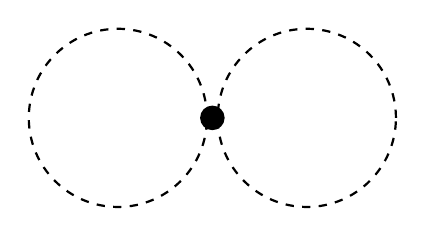
\begin{tikzpicture}
		[scale=0.4,inner sep=8mm, % this is the node radius
		vertex/.style={circle,thick,draw}, % this defines the default style for the vertex class
		thickedge/.style={line width=2pt}] % this defines the default style for the thick edges
		\node[vertex] (a1) at (0,0) [fill=white,dashed] {};
		\node[vertex] (a2) at (6,0) [fill=white,dashed] {};   
		\node[vertex] (a3) at (3,0) [inner sep=1mm,fill=black] {};           
		\end{tikzpicture}
	\end{center}
	\caption{Type~II of $G^*$.} \label{fig:TypeII}
\end{figure}
\medskip
\item [{\bf Type~III}:] Two cycles with at least two common vertices. In this case, $G^*$ can be derived from vertex dijsoint paths $P_a$, $P_b$, $P_c$ by first identifying one endvertex of each of these paths, and then identifying the other endvertices of these paths (see Figure~\ref{fig:TypeIII}).
\begin{figure}[h]
	\begin{center}
		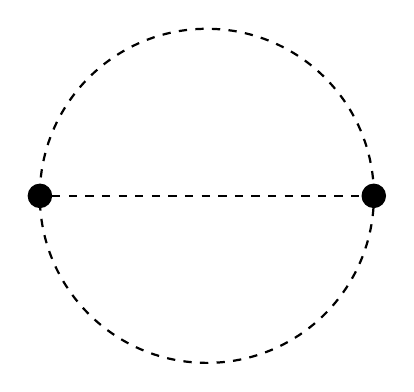
\begin{tikzpicture}
		[scale=0.4,inner sep=15.mm, % this is the node radius
		vertex/.style={circle,thick,draw}, % this defines the default style for the vertex class
		thickedge/.style={line width=2pt}] % this defines the default style for the thick edges
		\node[vertex] (a1) at (0,0) [fill=white,dashed] {};  
		\node[vertex] (a2) at (-5.3,0) [inner sep=1mm,fill=black] {};  
		\node[vertex] (a3) at (5.3,0) [inner sep=1mm,fill=black] {}; 
		%%
		\draw[thick,black, dashed] (a2)--(a3);      
		\end{tikzpicture}
	\end{center}
	\caption{Type~III of $G^*$.} \label{fig:TypeIII}
\end{figure}
\end{enumerate}

\medskip
We continue with some general lemmas that will simplify the computation of the number of connected sets in certain categories of graphs.

\begin{lemma}\label{Lem:identify}
Let $H$ be obtained from the disjoint union of graphs $H_1$ and $H_2$ by identifying a vertex $u_1$ in $H_1$ and a vertex $u_2$ in $H_2$ (similar to Figure~\ref{fig:TypeII}). We have
\begin{align*}
\N(H)=\N(H_1)+\N(H_2) -1 + (\N(H_1)_{u_1} -1 )(\N(H_2)_{u_2} -1 )\,.
\end{align*}
\end{lemma}

\begin{proof}
Let $u$ be the only common vertex of $H_1$ and $H_2$ in $H$. We have
\begin{align*}
\N(H-u)=\N(H_1-u_1)+\N(H_2-u_2)=\N(H_1)-\N(H_1)_{u_1} + \N(H_2)-\N(H_2)_{u_2}
\end{align*}
and 
\begin{align*}
\N(H)_u=\N(H_1)_{u_1}\cdot \N(H_2)_{u_2}\,.
\end{align*}
From these two identities, we get
\begin{align*}
\N(H)&=\N(H-u)+\N(H)_u\\
&=\N(H_1)-\N(H_1)_{u_1} + \N(H_2)-\N(H_2)_{u_2}+\N(H_1)_{u_1}\cdot \N(H_2)_{u_2}\\
&=\N(H_1)+\N(H_2) -1 + (\N(H_1)_{u_1} -1 )(\N(H_2)_{u_2} -1 )\,,
\end{align*}
which proves the lemma.
\end{proof}

\medskip

\begin{lemma}\label{Lemm:vtovprime}
Let $H$ be a graph, $v$ a pendant vertex and $v'$ its neighbour in $H$. Then
\begin{align*}
\N(H)=\N(H-v)+1+\N(H-v)_{v'}\,.
\end{align*}
\end{lemma}

\begin{proof}
The graph $H$ decomposes as in Lemma~\ref{Lem:identify}, where $H_1=vv'$ and $H_2=H-v$. Thus 
\begin{align*}
\N(H)=3 +\N(H-v) -1 + (2 -1 )(\N(H-v)_{v'} -1 )=\N(H-v)+1+\N(H-v)_{v'}\,.
\end{align*}
\end{proof}

\medskip
For an integer $m\geq 4$, we define the {\it tadpole} graph $D_m$ to be the unicyclic graph obtained by identifying one vertex of the cycle $C_3$ with one leaf of the path $P_{m-2}$. Furthermore, we define $L_n$ to be the graph $L_n:=G[3,3,n-4]$; see Figure~\ref{fig:TypeI}.

\begin{lemma}\label{Lem:FormLn}
We have 
\begin{align*}
\N(L_n)=\frac{(n+6)(n-1)}{2}
\end{align*}
for all $n\geq 5$.
\end{lemma}

\begin{proof}
It is easy to check that $\N(L_5)=22$. Let $n>5$, $v$ be the common vertex of a fixed $C_3$ and $P_{n-4}$ in $L_n$. The graph $L_n -v$ has $D_{n-3}$ as a connected component. It is proved in~\cite{Audacegenral2018} that 
\begin{align*}
\N(D_m)=\frac{(m-1)(m+4)}{2}
\end{align*}
for all $m\geq 3$. Thus
\begin{align*}
\N(L_n-v)=\N(P_2)+\N(D_{n-3})=3+ \frac{(n-4)(n+1)}{2}\,.
\end{align*}
Moreover, 
\begin{align*}
\N(L_n)_v=\N(C_3)_v \cdot \N(D_{n-2})_w\,,
\end{align*}
where $w$ is the unique pendant vertex of $D_{n-2}$. Since
\begin{align*}
\N(D_{n-2})_w=n-1\,, \quad \N(C_3)_v=4\,, 
\end{align*}
we deduce that $\N(L_n)_v=4(n-1)$ and that
\begin{align*}
\N(L_n)&=\N(L_n-v)+\N(L_n)_v\\
&=3+ \frac{(n-4)(n+1)}{2}+4(n-1)=\frac{(n+6)(n-1)}{2}\,,
\end{align*}
as needed.
\end{proof}

\medskip
Denote by $A_4$ the unique bicyclic graph on four vertices. For $n\geq 5$, we identify an endvertex of a $P_{n-3}$ with one vertex of degree two in $A_4$ to obtain $A_n \in \mathbb{B}_n$.

\begin{lemma}
We have
\begin{align*}
\N(A_n)=\frac{n^2+7n-16}{2}
\end{align*}
for all $n\geq 4$. In particular,
\begin{align*}
\N(L_5)=\N(A_5)=22\,, \quad \text{and} \quad \N(L_n)< \N(A_n) \quad \text{holds for all}~~~ n > 5\,.
\end{align*}

\end{lemma}
\begin{proof}
It is easy to check that $\N(A_4)=14$. For $n\geq 5$, denote by $u_1$ in $P_{n-3}$ and by $u_2$ in $A_4$ the two vertices that are identified to obtain $A_n$. We employ Lemma~\ref{Lem:identify} to get
\begin{align*}
\N(A_n)&=\N(P_{n-3})+\N(A_4) -1 + (\N(P_{n-3})_{u_1} -1 )(\N(A_4)_{u_2} -1 )\\
&=\binom{n-2}{2}+14-1+(n-3-1)(7-1)\\
&=\frac{(n-2)(n-3)}{2}+13+6(n-4)=\frac{n^2+7n-16}{2}\,.
\end{align*}
Now Lemma~\ref{Lem:FormLn} gives us
\begin{align*}
\N(A_n)-\N(L_n)=  \frac{n^2+7n-16}{2} -  \frac{(n+6)(n-1)}{2} = n-5 \geq 0
\end{align*}
for all $n\geq 5$, which proves the lemma.
\end{proof} 

\medskip
As a next step, we shall estimate the smallest number of connected sets containing a given vertex in a $n$-vertex bicyclic graph.

\begin{proposition}\label{Prop:nplus3}
If $G\in \mathbb{B}_n$ and $v\in V(G)$, then 
\begin{align*}
\N(G)_v \geq n+3\,.
\end{align*}
\end{proposition}

\begin{proof}
It is clear that $\N(A_4)_v=7$ if $v$ is of degree two, and  $\N(A_4)_v=8$ if $v$ is of degree three. So the proposition holds (with equality) for $n=4$. Henceforth, assume $n\geq 5$. We distinguish between three scenarios:
\begin{itemize}
\item $v$ is a pendant vertex of $G$, and $v'$ is the neighbour of $v$.\\
Since $G-v$ is also a bicyclic graph, we have
\begin{align*}
\N(G)_v=1+\N(G-v)_{v'} \geq 1+ (n-1+3)=n+3\,,
\end{align*}
where the inequality follows by induction on $n$.
\item $G$ contains a pendant vertex $u \neq v$.\\
Since $G-u$ is also a bicyclic graph, we have
\begin{align*}
\N(G)_v=\N(G-u)_v + \N(G)_{u,v} \geq (n-1+3)  + \N(G)_{u,v} \,,
\end{align*}
where the inequality follows by induction on $n$. The count for $\N(G)_{u,v}$ includes a shortest path between $u$ and $v$, thus $\N(G)_{u,v} \geq 1$. In particular,
\begin{align*}
\N(G)_v \geq  (n-1+3)  + 1 = n+3\,.
\end{align*}
\item $G$ does not have a pendant vertex.\\
All shortest paths starting at $v$ in $G$ contribute to the count $\N(G)_v$. Thus
$$\N(G)_v \geq n\,.$$
Vertex $v$ together with any two of its neighbours also induces a connected graph in which $v$ is not pendant. We deduce the following:
\begin{itemize}
\item If $v$ has at least three neighbours in $G$, then $\N(G)_v \geq n +3 +1$, where the final $1$ accounts for $G$ itself.
\item If $v$ has only two neighbours, say $v_1,v_2$ in $G$, then either $v_1$ or $v_2$ must have a neighbour, say $w$ not belonging to $\{v,v_1,v_2\}$. Thus, each of the graphs induced by $\{v,v_1,v_2\}$ and $\{v,v_1,v_2,w\}$ is connected and none of them has $v$ as a pendant vertex. Hence  $\N(G)_v \geq n +2 +1$, where the final $1$ accounts for the whole $G$.
\end{itemize}
\end{itemize}
This completes the proof of the proposition.
\end{proof}


\medskip
We list in Figure~\ref{fig:All5} all elements in the collection $\mathbb{B}_5$, alongside their numbers of connected sets (the details are omitted).
\begin{figure}[h]
	\begin{center}
		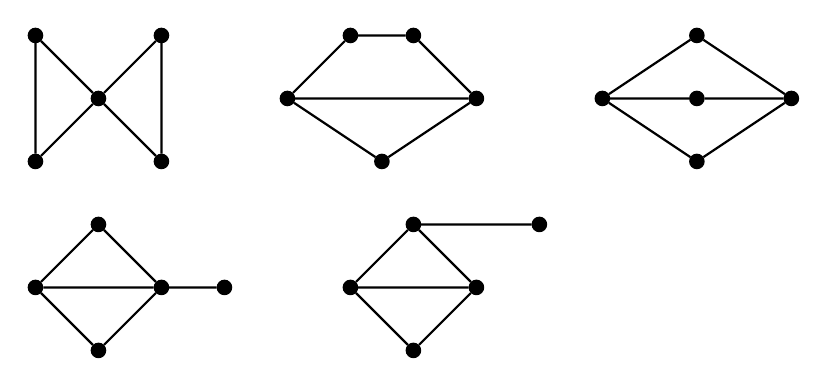
\begin{tikzpicture}
		[scale=0.4,inner sep=0.6mm, % this is the node radius
		vertex/.style={circle,thick,draw}, % this defines the default style for the vertex class
		thickedge/.style={line width=2pt}] % this defines the default style for the thick edges
		\node[vertex] (a1) at (0,2) [fill=black] {};  
		\node[vertex] (a2) at (0,-2) [fill=black] {};  
		\node[vertex] (a3) at (2,0) [fill=black] {}; 
		\node[vertex] (a4) at (4,2) [fill=black] {};  
		\node[vertex] (a5) at (4,-2) [fill=black] {}; 
		%%
		\draw[thick,black] (a1)--(a2) (a1)--(a3) (a2)--(a3) (a3)--(a4) (a3)--(a5) (a4)--(a5);      
		%%%%%%%%%%%%%%%%%
		\node[vertex] (b1) at (8,0) [fill=black] {};  
		\node[vertex] (b2) at (10,2) [fill=black] {};  
		\node[vertex] (b3) at (11,-2) [fill=black] {}; 
		\node[vertex] (b4) at (12,2) [fill=black] {};  
		\node[vertex] (b5) at (14,0) [fill=black] {}; 
		%%
		\draw[thick,black] (b1)--(b2) (b1)--(b3) (b1)--(b5) (b2)--(b4) (b3)--(b5) (b4)--(b5);      
		%%%%%%%%%%%%%%%%%
		\node[vertex] (c1) at (18,0) [fill=black] {};  
		\node[vertex] (c2) at (21,2) [fill=black] {};  
		\node[vertex] (c3) at (21,-2) [fill=black] {}; 
		\node[vertex] (c4) at (21,0) [fill=black] {};  
		\node[vertex] (c5) at (24,0) [fill=black] {}; 
		%%
		\draw[thick,black] (c1)--(c2) (c1)--(c3) (c1)--(c4) (c2)--(c5) (c3)--(c5) (c4)--(c5);
			%%%%%%%%%%%%%%%%%
		\node[vertex] (d1) at (0,-6) [fill=black] {};  
		\node[vertex] (d2) at (2,-4) [fill=black] {};  
		\node[vertex] (d3) at (2,-8) [fill=black] {}; 
		\node[vertex] (d4) at (4,-6) [fill=black] {};  
		\node[vertex] (d5) at (6,-6) [fill=black] {}; 
		%%
		\draw[thick,black] (d1)--(d2) (d1)--(d3) (d1)--(d4) (d2)--(d4) (d3)--(d4) (d4)--(d5);
			%%%%%%%%%%%%%%%%%
		\node[vertex] (e1) at (10,-6) [fill=black] {};  
		\node[vertex] (e2) at (12,-4) [fill=black] {};  
		\node[vertex] (e3) at (12,-8) [fill=black] {}; 
		\node[vertex] (e4) at (14,-6) [fill=black] {};  
		\node[vertex] (e5) at (16,-4) [fill=black] {}; 
		%%
	\draw[thick,black] (e1)--(e2) (e1)--(e3) (e1)--(e4) (e2)--(e4) (e3)--(e4) (e2)--(e5);      
		\end{tikzpicture}
	\end{center}
	\caption{All bicyclic graphs on five vertices. Their numbers of connected sets are $22,~24,~26,~23,~22$, respectively.} \label{fig:All5}
\end{figure}


\medskip
We are now ready to state and prove our first theorem.

\begin{theorem}
Let $n>4$ and $G\in \mathbb{B}_n$. It holds that
$$\N(G) \geq \N(L_n)=\frac{(n+6)(n-1)}{2}
\,.$$ Equality happens in the case where $n>5$ if and only if $G$ is isomorphic to $L_n$. 
\end{theorem}

\begin{proof}
The formula for $\N(L_n)$ is given in Lemma~\ref{Lem:FormLn}. If $n=5$, then $\N(G) \geq 22$ by Figure~\ref{fig:All5}. Equality holds if and only if $G=L_5$ or $G=A_5$. Let $n>5$, and assume that $G$ has a pendant vertex, say $v$. Then $G-v \in \mathbb{B}_{n-1}$ and the induction hypothesis on $n$ yields
\begin{align*}
\N(G-v) \geq \frac{(n-1+6)(n-1-1)}{2}\,.
\end{align*}
This implies that
\begin{align*}
\N(G)=\N(G-v)+\N(G)_v \geq \frac{(n+5)(n-2)}{2}+ (n+3)\,,
\end{align*}
now using Proposition~\ref{Prop:nplus3}. Hence
\begin{align*}
\N(G)\geq \frac{(n+5)(n-2)}{2}+ (n+3) > \frac{(n+5)(n-2)}{2}+ (n+2)=\frac{(n+6)(n-1)}{2}\,,
\end{align*}
and we are done in this case. If $G$ does not have a pendant vertex, then $G=G^*$ is one of the three types in Figures~\ref{fig:TypeI},~\ref{fig:TypeII},~\ref{fig:TypeIII}. Henceforth, we assume that $G\in \mathbb{B}_n$ has the smallest number of connected sets. 

{\sc Claim~1}: $G$ cannot be of type II.\\
Suppose not. Replace the cycle $C_q$ ($q\geq p$) in $G=G^*=G[p,q,n+2-p-q]$ with the tadpole graph $D_q$, as shown in Figure~\ref{fig:FromTypeII}, to obtain a graph $G'\in \mathbb{B}_n$. By $q\geq p$, we necessarily have $q\geq 4$.
\begin{figure}[h]
	\begin{center}
		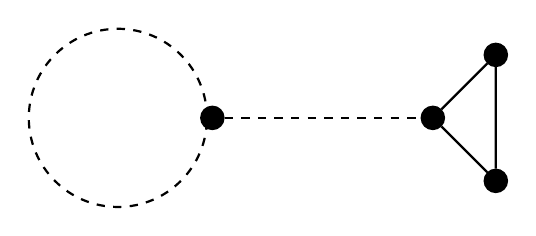
\begin{tikzpicture}
		[scale=0.4,inner sep=8mm, % this is the node radius
		vertex/.style={circle,thick,draw}, % this defines the default style for the vertex class
		thickedge/.style={line width=2pt}] % this defines the default style for the thick edges
		\node[vertex] (a1) at (0,0) [fill=white,dashed] {};
		\node[vertex] (b1) at (10,0) [inner sep=1mm,fill=black] {};  
		\node[vertex] (b2) at (12,2) [inner sep=1mm,fill=black] {};   
		\node[vertex] (b3) at (12,-2) [inner sep=1mm,fill=black] {};   
		\node[vertex] (a3) at (3,0) [inner sep=1mm,fill=black] {};     
	\draw[thick,black, dashed] (a3)--(b1) ;   
	\draw[thick,black] (b1)--(b2) (b1)--(b3) (b2)--(b3);      
		\end{tikzpicture}
	\end{center}
	\caption{From Type~II to a Type~I.} \label{fig:FromTypeII}
\end{figure}
It follows from Lemma~\ref{Lem:identify} that
\begin{align*}
\N(G')-\N(G)=\N(D_q)-\N(C_q) + (\N(D_q)_{u_1} - \N(C_q)_{u_2} )(\N(C_p)_{u_2} -1 )\,,
\end{align*}
where $u_1$ is the unique pendant vertex in $D_q$. It is shown in~\cite{Audacegenral2018} that $D_m$ uniquely minimises the number of connected sets over the set of all $m$-vertex unicyclic graphs. Therefore,
\begin{align*}
\N(G')-\N(G) < (\N(D_q)_{u_1} - \N(C_q)_{u_2} )(\N(C_p)_{u_2} -1 )\,.
\end{align*}
Since $\N(D_q)_{u_1}=q+1$, while $\N(C_q)_{u_2}=1+\binom{q}{2}$, we deduce that
$$\N(D_q)_{u_1} - \N(C_q)_{u_2} < 0\,,$$
and that $\N(G')-\N(G) < 0$. This contradicts the minimality of $G$ with respect to the number of connected sets, thus proving the claim.

\medskip
{\sc Claim~2}: $G$ cannot be of type III.\\
Suppose not. By construction (see Figure~\ref{fig:TypeIII}), $G=G^*$ has no cut vertex (i.e. $G-u$ is still connected for every $u\in \V(G)$). We proved in~\cite{AudaceCut2019} that $C_n$ is the unique graph having the smallest number of connected sets among all $n$-vertex connected graphs with no cut vertex. Thus $\N(G) > \N(C_n)$. On the other hand, 
\begin{align*}
\N(C_n) - \N(L_n) = n^2-n+1 - \frac{(n+6)(n-1)}{2} = \frac{n^2 -7n +8}{2}\,,
\end{align*}
which is positive for all $n>5$. Therefore, $\N(G) > \N(C_n) > \N(L_n)$. In particular, $G$ cannot reach the smallest number of connected sets over $\mathbb{B}_n$. This proves Claim~2.

\medskip
As a consequence of the above two Claims, a graph $G\in \mathbb{B}_n$ that minimises the number of connected sets must be of type~I.

{\sc Claim~3}: $G$ is isomorphic to $L_n$.\\
Suppose not. Replace the cycle $C_q$ ($q\geq p$) in $G=G^*$ (see Figure~\ref{fig:TypeI}) with the tadpole graph $D_q$ to obtain the same shape $G'$, as shown in Figure~\ref{fig:FromTypeII}. Using Lemma~\ref{Lem:identify}, we obtain
\begin{align*}
\N(G')-\N(G) = \N(D_q)-\N(C_q) + (\N(D_q)_{u_1} - \N(C_q)_{u_2} ) \big(\N (G - (V(C_q)\backslash \{u_2\}))_{u_2} -1 \big) \,,
\end{align*}
where $u_1$ is the unique pendant vertex of $D_q$. Since $\N(D_q)_{u_1} - \N(C_q)_{u_2} \leq 0$ and $D_m$ is the only $m$-vertex unicyclic graph with the smallest number of connected sets, we deduce that $\N(G')-\N(G) < 0$.

If $p=3$ then $G'$ is isomorphic to $L_n$. Otherwise, we apply the same graph transformation to $G'$ (replacing $C_p$ with $D_p$) to obtain $G''$. Hence  $\N(G'') < \N(G') < \N(G)$. Since $G''$ is isomorphic to $L_n$, the proof of the claim (thus also the theorem) is finished.
\end{proof}

\medskip
In what follows, we shift our focus on the maximisation problem. For our purposes, we shall even determine both the largest and the second-largest numbers of connected sets over $\mathbb{B}_n$, for all $n\geq 8$.

\medskip
Let $n\geq 6$ be an integer. Starting with two vertex disjoint cycles $C_3$ and $C_3$, first identify one vertex in a $C_3$ and one vertex in the other $C_3$ by vertex $w$, and then attach $n-5$ pendant edges to $w$. We denote the resulting graph by $R_n$. Clearly, $R_n \in \mathbb{B}_n$.

Similarly, we define $B_n$ to be the graph constructed from $A_4$ by attach $n-4$ pendant edges to the same vertex $w$ of degree $3$ in $A_4$. Clearly, $B_n \in \mathbb{B}_n$.

As usual, the $n$-vertex star graph is denoted by $S_n$.

\begin{lemma}\label{Form:RnBn}
We have
\begin{align*}
\N(R_n)&=n+1+2^{n-1}\\
\N(B_n)&=n+2+2^{n-1} =\N(R_n) +1
\end{align*}
for all $n\geq 6$.
\end{lemma}

\begin{proof}
The graph $R_n-w$ consists of two copies of $P_2$ and $n-5$ copies of $P_1$, while $w$ is adjacent to all other vertices of $R_n$. Thus
\begin{align*}
\N(R_n)=\N(R_n)_w + \N(R_n-w)=2^{n-1}+ 2\N(P_2)+ n-5=2^{n-1}+n+1\,.
\end{align*}
By Lemma~\ref{Lem:identify},
\begin{align*}
\N(B_n)=\N(A_4)+\N(S_{n-3}) -1 + (\N(A_4)_w -1 )(\N(S_{n-3})_w -1 )\,,
\end{align*}
where $w$ is also the center of the star. Thus
\begin{align*}
\N(B_n)=14 +(2^{n-4}+n-4) -1 + (8 -1 )(2^{n-4}-1 )=2^{n-1}+n+2\,,
\end{align*}
as stated.
\end{proof}

\medskip
We shall prove that $B_n$ uniquely maximises the number of connected sets among all $n$-vertex bicyclic graphs, provided $n>7$. Henceforth, we assume $n\geq 8$.

\medskip

Lemma~\ref{singleBranch} below is an important tool to proving our second theorem. It already appeared in~\cite{AudaceGirth2018,AudTOUT}.

\begin{lemma}[\cite{AudaceGirth2018,AudTOUT}]\label{singleBranch}
	Let $L,M,R$ be three non-trivial connected graphs whose vertex sets are pairwise disjoints. Let $l \in V(L),~ r\in V(R)$ and $u,v \in V(M)$ be fixed vertices such that $u \neq v$. Denote by $G$ the graph obtained from $L,M,R$ by identifying $l$ with $u$, and $r$ with $v$. Similarly, let $G'$ (resp. $G''$) be the graph obtained from $L,M,R$ by identifying both $l,r$ with $u$ (resp. both $l,r$ with $v$); see Figure~\ref{diagGGpGpp} for a diagram of these graphs.
	\begin{figure}[htbp]\centering
		\definecolor{qqqqff}{rgb}{0.,0.,1.}
		\resizebox{0.7\textwidth}{!}{%
		\begin{tikzpicture}[line cap=round,line join=round,>=triangle 45,x=1.0cm,y=1.0cm]
		rectangle (17.25469285535401,15.543118314192673);
		\draw [dash pattern=on 2pt off 2pt] (8.02,12.78)-- (10.02,12.78);
		\draw [dash pattern=on 2pt off 2pt] (10.02,12.78)-- (10.,12.);
		\draw [dash pattern=on 2pt off 2pt] (10.,12.)-- (10.02,11.26);
		\draw [dash pattern=on 2pt off 2pt] (10.02,11.26)-- (8.,11.26);
		\draw [dash pattern=on 2pt off 2pt] (8.,11.26)-- (8.,12.);
		\draw [dash pattern=on 2pt off 2pt] (8.,12.)-- (8.02,12.78);
		\draw [dash pattern=on 2pt off 2pt] (6.48,12.56)-- (8.,12.);
		\draw [dash pattern=on 2pt off 2pt] (6.48,11.48)-- (8.,12.);
		\draw [dash pattern=on 2pt off 2pt] (6.48,12.56)-- (6.48,11.48);
		\draw [dash pattern=on 2pt off 2pt] (10.,12.)-- (11.48,12.48);
		\draw [dash pattern=on 4pt off 4pt] (10.,12.)-- (11.46,11.46);
		\draw [dash pattern=on 2pt off 2pt] (11.48,12.48)-- (11.46,11.46);
		\draw (8.002875389073733,12.308886980787792) node[anchor=north west] {$l,u$};
		\draw (9.126357554291436,12.19457622267538) node[anchor=north west] {$v,r$};
		\draw (6.736460949518799,12.287683803799489) node[anchor=north west] {$L$};
		\draw (10.70036563986977,12.304751529462257) node[anchor=north west] {$R$};
		\draw [dash pattern=on 2pt off 2pt] (4.,10.)-- (6.,10.);
		\draw [dash pattern=on 2pt off 2pt] (6.,10.)-- (5.98,9.22);
		\draw [dash pattern=on 2pt off 2pt] (5.98,9.22)-- (6.,8.48);
		\draw [dash pattern=on 2pt off 2pt] (6.,8.48)-- (3.98,8.48);
		\draw [dash pattern=on 2pt off 2pt] (3.98,8.48)-- (3.98,9.22);
		\draw [dash pattern=on 2pt off 2pt] (3.98,9.22)-- (4.,10.);
		\draw [dash pattern=on 2pt off 2pt] (3.12,10.28)-- (3.98,9.22);
		\draw [dash pattern=on 2pt off 2pt] (2.6,9.6)-- (3.98,9.22);
		\draw [dash pattern=on 2pt off 2pt] (3.12,10.28)-- (2.6,9.6);
		\draw (4.031552359486242,9.502599906980058) node[anchor=north west] {$l,u,r$};
		\draw (6.006612285785838,9.41691066509247) node[anchor=north west] {$v$};
		\draw (3.008420807842294,10.0050302314765) node[anchor=north west] {$L$};
		\draw (3.087042324067116,8.845683517584332) node[anchor=north west] {$R$};
		\draw [dash pattern=on 2pt off 2pt] (12.,10.)-- (14.,10.);
		\draw [dash pattern=on 2pt off 2pt] (14.,10.)-- (13.98,9.22);
		\draw [dash pattern=on 2pt off 2pt] (13.98,9.22)-- (14.,8.48);
		\draw [dash pattern=on 2pt off 2pt] (14.,8.48)-- (11.98,8.48);
		\draw [dash pattern=on 2pt off 2pt] (11.98,8.48)-- (11.98,9.22);
		\draw [dash pattern=on 2pt off 2pt] (11.98,9.22)-- (12.,10.);
		\draw [dash pattern=on 2pt off 2pt] (13.98,9.22)-- (14.9,10.32);
		\draw [dash pattern=on 4pt off 4pt] (13.98,9.22)-- (15.42,9.66);
		\draw [dash pattern=on 2pt off 2pt] (14.9,10.32)-- (15.42,9.66);
		\draw (12.000266144323993,9.432599906980058) node[anchor=north west] {$u$};
		\draw (12.761465421630708,9.532775213766935) node[anchor=north west] {$v,l,r$};
		\draw (14.542891846445562,10.147962505813732) node[anchor=north west] {$R$};
		\draw [dash pattern=on 2pt off 2pt] (2.66,8.42)-- (3.98,9.22);
		\draw [dash pattern=on 2pt off 2pt] (3.44,7.86)-- (3.98,9.22);
		\draw [dash pattern=on 2pt off 2pt] (2.66,8.42)-- (3.44,7.86);
		\draw (8.654102536581874,12.838560337733874) node[anchor=north west] {$M$};
		\draw (4.70415799076956,10.0550302314765) node[anchor=north west] {$M$};
		\draw (12.718182533719721,10.0550302314765) node[anchor=north west] {$M$};
		\draw [dash pattern=on 2pt off 2pt] (13.98,9.22)-- (15.44,8.52);
		\draw [dash pattern=on 2pt off 2pt] (14.78,7.92)-- (13.98,9.22);
		\draw [dash pattern=on 2pt off 2pt] (15.44,8.52)-- (14.78,7.92);
		\draw [dash pattern=on 2pt off 2pt] (15.44,8.52)-- (14.78,7.92);
		\draw [dash pattern=on 2pt off 2pt] (15.44,8.52)-- (14.78,7.92);
		\draw (14.521338055883508,8.817237308146387) node[anchor=north west] {$L$};
		\draw (8.682548746019819,11.18282315480661) node[anchor=north west] {$G$};
		\draw (4.618293442095093,8.37342849987477) node[anchor=north west] {$G'$};
		\draw (12.675250259382487,8.330496225537535) node[anchor=north west] {$G''$};
		
		\draw [fill=black] (8.02,12.78) circle (0.5pt);
		\draw [fill=black] (10.02,12.78) circle (0.5pt);
		\draw [fill=black] (8.,11.26) circle (0.5pt);
		\draw [fill=black] (10.02,11.26) circle (0.5pt);
		\draw [fill=black] (8.,12.) circle (2.0pt);
		\draw [fill=black] (10.,12.) circle (2.0pt);
		\draw [fill=black] (6.48,12.56) circle (0.5pt);
		\draw [fill=black] (6.48,11.48) circle (0.5pt);
		\draw [fill=qqqqff] (11.48,12.48) circle (0.5pt);
		\draw [fill=qqqqff] (11.46,11.46) circle (0.5pt);
		\draw [fill=black] (4.,10.) circle (0.5pt);
		\draw [fill=black] (6.,10.) circle (0.5pt);
		\draw [fill=black] (3.98,8.48) circle (0.5pt);
		\draw [fill=black] (6.,8.48) circle (0.5pt);
		\draw [fill=black] (3.98,9.22) circle (2.0pt);
		\draw [fill=black] (5.98,9.22) circle (2.0pt);
		\draw [fill=black] (3.12,10.28) circle (0.5pt);
		\draw [fill=black] (2.6,9.6) circle (0.5pt);
		\draw [fill=black] (12.,10.) circle (0.5pt);
		\draw [fill=black] (14.,10.) circle (0.5pt);
		\draw [fill=black] (11.98,8.48) circle (0.5pt);
		\draw [fill=black] (14.,8.48) circle (0.5pt);
		\draw [fill=black] (11.98,9.22) circle (2.0pt);
		\draw [fill=black] (13.98,9.22) circle (2.0pt);
		\draw [fill=black] (15.44,8.52) circle (0.5pt);
		\draw [fill=black] (14.78,7.92) circle (0.5pt);
		\draw [fill=qqqqff] (14.9,10.32) circle (0.5pt);
		\draw [fill=qqqqff] (15.42,9.66) circle (0.5pt);
		\draw [fill=black] (3.44,7.86) circle (0.5pt);
		\draw [fill=black] (2.66,8.42) circle (0.5pt);
		\end{tikzpicture}}
		\caption{The graphs $G,G',G''$ constructed in Lemma~\ref{singleBranch}.}\label{diagGGpGpp}
	\end{figure}

We have 
\begin{align*}
	\N(G') - \N(G)&= (\N(R)_r -1) (\N(L)_l \cdot \N(M-v)_u - \N(M-u)_v)\,,\\
	\N(G'') - \N(G)&= (\N(L)_l -1) (\N(R)_r \cdot \N(M-u)_v - \N(M-v)_u)\,,
	\end{align*}
	In particular, it holds that
	\begin{align*}
	\N(G') > \N(G) ~~ \text{or} ~~ \N(G'') > \N(G)\,.
	\end{align*}
\end{lemma}

\medskip
The next proposition is fairly well-known, see for instance~\cite{Audacegenral2018,Wang2005}.

\begin{proposition}\label{upperTr}
Let $T$ be a tree on $n$ vertices whose root is $v$. Then $\N(T)_v\leq 2^{n-1}$. Equality holds if and only if $T$ is the star $S_n$ and $v$ is the center of $T$.
\end{proposition}

\medskip
Let $n>2$ and $Q_n$ be the graph that results from adding one edge between two leaves of the star $S_n$. Clearly, $Q_n$ contains only one cycle, which is $C_3$. 

\medskip
The largest and second-largest bicyclic graphs with respect to the number of connected sets are completely described in the next theorem.

\begin{theorem}
Let $n\geq 8$ and $G \in \mathbb{B}_n$. Then
$$\N(G) \leq \N(B_n)\,,$$
with equality if and only if $G$ is isomorphic to $B_n$. Moreover,
$$\N(G) \leq \N(R_n)$$ holds for all $G\in \mathbb{B}_n \backslash \{B_n\}$.
\end{theorem}

\begin{proof}
Let $n\geq 8$ and $G_0 \in \mathbb{B}_n$. By Lemma~\ref{Gstar}, $G_0$ can be obtained from its bicyclic subgraph $G_0^*$ by attaching trees at the vertices of $G_0^*$. We make the specialisation $M:=G_0^*$ and repeatedly apply Lemma~\ref{singleBranch}, until we get a new graph $G_1\in \mathbb{B}_n$ that can also be constructed from $G_1^*=G_0^*$ by attaching (possibly none) a tree $T_1$ rooted at only one vertex, say $v$ of $G_1^*$. Thus, $\N(G_1)\geq \N(G_0)$, with equality if and only if $G_1$ is isomorphic to $G_0$.

\medskip
Consider the bicyclic graph $G_1$. As was described in Lemma~\ref{Lem:identify}, `replace' the tree $T_1$ with the star $S_{|V(T_1)|}$ whose center is $v$, to obtain a graph $G_2\in \mathbb{B}_n$. This gives us
\begin{align*}
\N(G_2)-\N(G_1)=\N(S_{|V(T_1)|}) - \N(T_1) + (\N(S_{|V(T_1)|})_{v} - \N(T_1)_v)(\N(G_1^*)_{v} -1 )\,.
\end{align*}
It is a folklore statement that $S_m$ uniquely reaches the maximum number of connected sets among all $m$-vertex trees. Together with Proposition~\ref{upperTr}, we deduce that $\N(G_2) \geq \N(G_1)$, with equality if and only if $T_1$ is a star and $v$ its center.

\medskip
Consider $G_2$, and let us first focus on its subgraph $G_2^*=G_1^*=G_0^*$.
\begin{itemize}
\item Assume $G_2^*$ is of type~I or type~II (see Figures~\ref{fig:TypeI} and~\ref{fig:TypeII} with $q\geq p$), and let $H:=G_2^* - (V(C_p) \backslash u)$, where $u$ is the unique common vertex of $C_p$ and $H$ in $G_2^*$. As long as $|V(H)|\geq 5$, `replace' the part $H$ of $G_2^*$ with the graph $Q_{|V(H)|}$ to obtain a graph $G'_3\in \mathbb{B}_n$, as shown in Figure~\ref{fig:TypeIorIItoQ}.
\begin{figure}[h]
	\begin{center}
		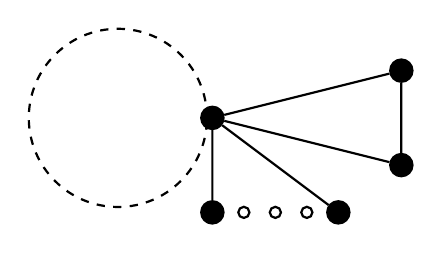
\begin{tikzpicture}
		[scale=0.4,inner sep=8mm, % this is the node radius
		vertex/.style={circle,thick,draw}, % this defines the default style for the vertex class
		thickedge/.style={line width=2pt}] % this defines the default style for the thick edges
		\node[vertex] (a1) at (0,0) [fill=white,dashed] {};
		\node[vertex] (b1) at (3,0) [inner sep=1mm,fill=black] {};  
	%	\node[vertex] (l) at (3.3,0.9) [inner sep=0.15mm, fill=none] {$u$};  
		\node[vertex] (b2) at (9,1.5) [inner sep=1mm,fill=black] {};   
		\node[vertex] (b3) at (9,-1.5) [inner sep=1mm,fill=black] {};   
		%\node[vertex] (a3) at (3,0) [inner sep=1mm,fill=black] {};     
	%\draw[thick,black, dashed] (a3)--(b1) ;   
	\node[vertex] (c1) at (3,-3) [inner sep=1mm,fill=black] {}; 
	\node[vertex] (d) at (4,-3) [inner sep=0.5mm,fill=white] {}; 
		\node[vertex] (e) at (5,-3) [inner sep=0.5mm,fill=white] {}; 
		\node[vertex] (f) at (6,-3) [inner sep=0.5mm,fill=white] {}; 
	\node[vertex] (c2) at (7,-3) [inner sep=1mm,fill=black] {};  
	\draw[thick,black] (b1)--(b2) (b1)--(b3) (b2)--(b3);     
	\draw[thick,black] (b1)--(c1) (b1)--(c2);      
		\end{tikzpicture}
	\end{center}
	\caption{Replacing part $H$ of Type~I or Type~II with $Q_{|V(H)|}$ to obtain $G'_3\in \mathbb{B}_n$.} \label{fig:TypeIorIItoQ}
\end{figure}
Vertex $u$ is adjacent to all other vertices in $Q_{|V(H)|}$, thus $\N(Q_{|V(H)|})_u=2^{|V(H)| -1}$. On the other hand, it was proved in~\cite{Audacegenral2018} that $Q_m$ uniquely maximises the number of connected sets among all unicyclic graphs of order $m>5$. Hence Lemma~\ref{Lem:identify} implies that $\N(G'_3) > \N(G^*_2)$, provided $|V(H)|>5$. However, if $m=5$ then $Q_5$ and $C_5$ are the only $m$-vertex unicyclic graphs with the maximum number of connected sets. By $q\geq p \geq 3$, vertex $u$ cannot be adjacent to all other vertices of $H$, unless $q=3$ (i.e. $G_2$ is isomorphic to $R_n$). Assume then $q>3$. It follows again by Lemma~\ref{Lem:identify} that $\N(G'_3) > \N(G^*_2)$ in the case where $|V(H)|=5$.

Whenever necessary, we can apply, provided $p\geq 5$, this same transformation on the part $C_p$ of $G'_3$ to obtain the graph $R_{|V(G'_3)|}$ and the inequality $\N(R_{|V(G'_3)|}) > \N(G'_3)$. Hence 
\begin{align*}
\N(R_{|V(G'_3)|}) > \N(G'_3) > \N(G^*_2) \quad \text{and} \quad \N(G_2) \geq \N(G_1) \geq \N(G_0)\,.
\end{align*}
We are left with the situation where $|V(H)|\leq 4$ and $p\leq 4$ hold simultaneously in the graph $G_2^*=G_0^*$. All such graphs $G_2^*$ are shown in Figure~\ref{fig:H4p4}.
\begin{figure}[h]
	\begin{center}
		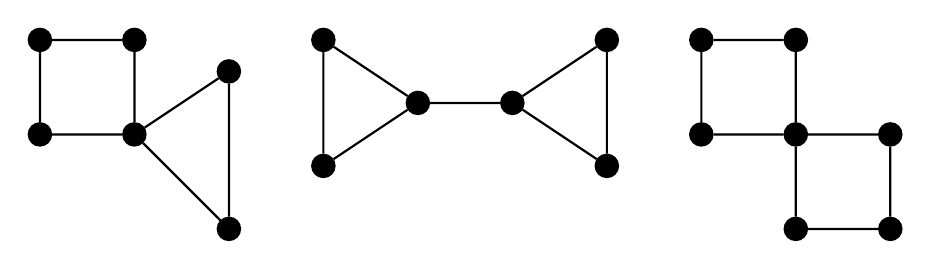
\begin{tikzpicture}
		[scale=0.4,inner sep=8mm, % this is the node radius
		vertex/.style={circle,thick,draw}, % this defines the default style for the vertex class
		thickedge/.style={line width=2pt}] % this defines the default style for the thick edges
		\node[vertex] (a1) at (0,0) [inner sep=1mm,fill=black] {};
		\node[vertex] (a2) at (3,0) [inner sep=1mm,fill=black] {};  
		\node[vertex] (a3) at (0,-3) [inner sep=1mm,fill=black] {};   
		\node[vertex] (a4) at (3,-3) [inner sep=1mm,fill=black] {};   
		\node[vertex] (a5) at (6,-1) [inner sep=1mm,fill=black] {};   
		\node[vertex] (a6) at (6,-6) [inner sep=1mm,fill=black] {};   
\draw[thick,black] (a1)--(a2) (a1)--(a3) (a2)--(a4) (a3)--(a4) (a4)--(a5) (a4)--(a6) (a5)--(a6);     
%%%%%%%%%%%%%%%%%%
\node[vertex] (b1) at (9,0) [inner sep=1mm,fill=black] {};
		\node[vertex] (b2) at (9,-4) [inner sep=1mm,fill=black] {};  
		\node[vertex] (b3) at (12,-2) [inner sep=1mm,fill=black] {}; 
		\node[vertex] (b4) at (15,-2) [inner sep=1mm,fill=black] {};
		\node[vertex] (b5) at (18,0) [inner sep=1mm,fill=black] {};   
			\node[vertex] (b6) at (18,-4) [inner sep=1mm,fill=black] {};   
			\draw[thick,black] (b1)--(b2) (b1)--(b3) (b2)--(b3) (b3)--(b4) (b4)--(b5) (b4)--(b6) (b5)--(b6);     
			%%%%%%%%%%%%%%%%%%
\node[vertex] (c1) at (21,0) [inner sep=1mm,fill=black] {};
		\node[vertex] (c2) at (24,0) [inner sep=1mm,fill=black] {};  
		\node[vertex] (c3) at (21,-3) [inner sep=1mm,fill=black] {};   
		\node[vertex] (c4) at (24,-3) [inner sep=1mm,fill=black] {};   
		\node[vertex] (c7) at (27,-3) [inner sep=1mm,fill=black] {};   
		\node[vertex] (c5) at (24,-6) [inner sep=1mm,fill=black] {}; 
		\node[vertex] (c8) at (27,-6) [inner sep=1mm,fill=black] {}; 
		\draw[thick,black] (c1)--(c2) (c1)--(c3) (c2)--(c4) (c3)--(c4) (c4)--(c5) (c4)--(c7) (c5)--(c8) (c7)--(c8);     
%%%%%%%%%%%%%%%%%
		\end{tikzpicture}
	\end{center}
	\caption{All graphs $G_2^*=G_0^*$ corresponding to the case where $|V(H)|\leq 4$ and $p\leq 4$. These graphs contain precisely $37,~30,~61$ connected sets, respectively.} \label{fig:H4p4}
\end{figure}

Recall that $G_2 \in \mathbb{B}_n$ can be constructed from $G_2^*=G_0^*$ by attaching (possibly none) a star $S_r$ rooted at only one vertex, say $v$ of $G_2^*$. In view of Lemma~\ref{Form:RnBn}, 
\begin{align*}
\N(R_6)=39 > 37\,, \quad \N(R_7)=72 > 61\,.
\end{align*} 
In this case where $G_2^*$ is one of the graph shown in Figure~\ref{fig:H4p4}, we `replace' $G_2^*$ directly with $R_{|V(G_2^*)|}$ in $G_2$ to obtain the graph $R_n$. Therefore, Lemma~\ref{Lem:identify} combined with
\begin{align*}
\N(R_{|V(G_2^*)|}) > \N(G^*_2) \quad \text{and} \quad \N(G_2) \geq \N(G_1) \geq \N(G_0)
\end{align*}
give us $\N(R_n) > \N(G_2) \geq \N(G_1) \geq \N(G_0)$, and we are done.

\medskip
\item Assume $G_2^*$ is of type~III (see Figure~\ref{fig:TypeIII}). Then $G_2^*$ can be obtained from vertex disjoint paths $P_a$, $P_b$, $P_c$ by first identifying one endvertex of each of these paths, and then identifying the other endvertices of these paths. Thus $2\leq a\leq b \leq c$ and $b\geq 3$. Set $m:=|V(G^*_2)|$.

First, assume $c\geq 5$. Let $v$ be a vertex of $G_2^*$ such that $v_1', v_1, v, v_2, v_2'$ are five consecutive vertices on the path $P_c$. We extract certain categories of vertex subsets of $G_2^*$, each of which contains $v$:
\begin{itemize}
\item The union of $\{v\}$ and any nonempty subset of $V(G_2^*)\backslash \{v_1,v_2\}$; there are $2^{m-3}-1$ of them;
\item The union of $\{v,v_2\}$ and any nonempty subset of $V(G_2^*)\backslash \{v_1,v'_2\}$; there are $2^{m-4}-1$ of them;
\item The union of $\{v,v_1\}$ and any nonempty subset of $V(G_2^*)\backslash \{v_2,v'_1\}$; there are $2^{m-4}-1$ of them;
\item The union of $\{v,v_1,v_2\}$ and any nonempty subset of $V(G_2^*)\backslash \{v'_1,v'_2\}$; there are $2^{m-5}-1$ of them.
\end{itemize}
Each of the above subset of $V(G_2^*)$ contains $v$ and induces a disconnected graph. Consequently,
\begin{align*}
\N(G_2^*)_v \leq &2^{m-1} - (2^{m-3}-1) - (2^{m-4}-1) - (2^{m-4}-1) - (2^{m-5}-1)\\
&=2^{m-2}+4-2^{m-5} \leq 2^{m-2} +2\,,
\end{align*}
since $m\geq c+1 >5$. On the other hand, $\N(G_2^* -v) < \N(Q_{m-1})$, since $G_2^* -v$ is a unicyclic graph on $m-1$ vertices, which is not isomorphic to $Q_{m-1}$ or $C_5$.

Fix $z$, a vertex of degree $2$, belonging to a $C_3$ in $R_m$, and let $z'$ be the unique neigbhour of $z$ that lies on the other $C_3$ ($z'$ is adjacent to all other vertices of $R_m$). Then
\begin{align*}
\N(R_m)_z=\N(R_m)_{z,z'}+ \N(R_m-z')_z=2^{m-2}+2\,.
\end{align*} 
Hence
\begin{align*}
\N(R_m)&=\N(R_m)_z + \N(R_m-z) =\N(R_m)_z + \N(Q_{m-1}) =  2+2^{m-2} + \N(Q_{m-1}) \\
& >2+ 2^{m-2} + \N(G_2^* -v) \geq \N(G_2^*)_v + \N(G_2^* -v) = \N(G_2^*)\,.
\end{align*}
Recall that $G_2 \in \mathbb{B}_n$ can be derived from $G_2^*$ by attaching (possibly none) a star $S_{n-m}$ centered at only one vertex, say $v$ of $G_2^*$. Now `replace' $G_2^*$ with $R_m$ to obtain the graph $R_n$. We therefore infer from Lemma~\ref{Lem:identify} together with
\begin{align*}
\N(G_2) \geq \N(G_1) \geq \N(G_0)
\end{align*}
that $\N(R_n) > \N(G_2) \geq \N(G_1) \geq \N(G_0)$, and we are done with the case where $c\geq 5$. To finish the proof of the theorem, we need to rule out the case where $c\leq 4$ (thus $2\leq a \leq b \leq c \leq 4$). In this case $|V(G_2^*)| \leq 8$, see Figure~\ref{fig:2abc4}.
\begin{figure}[h]
	\begin{center}
		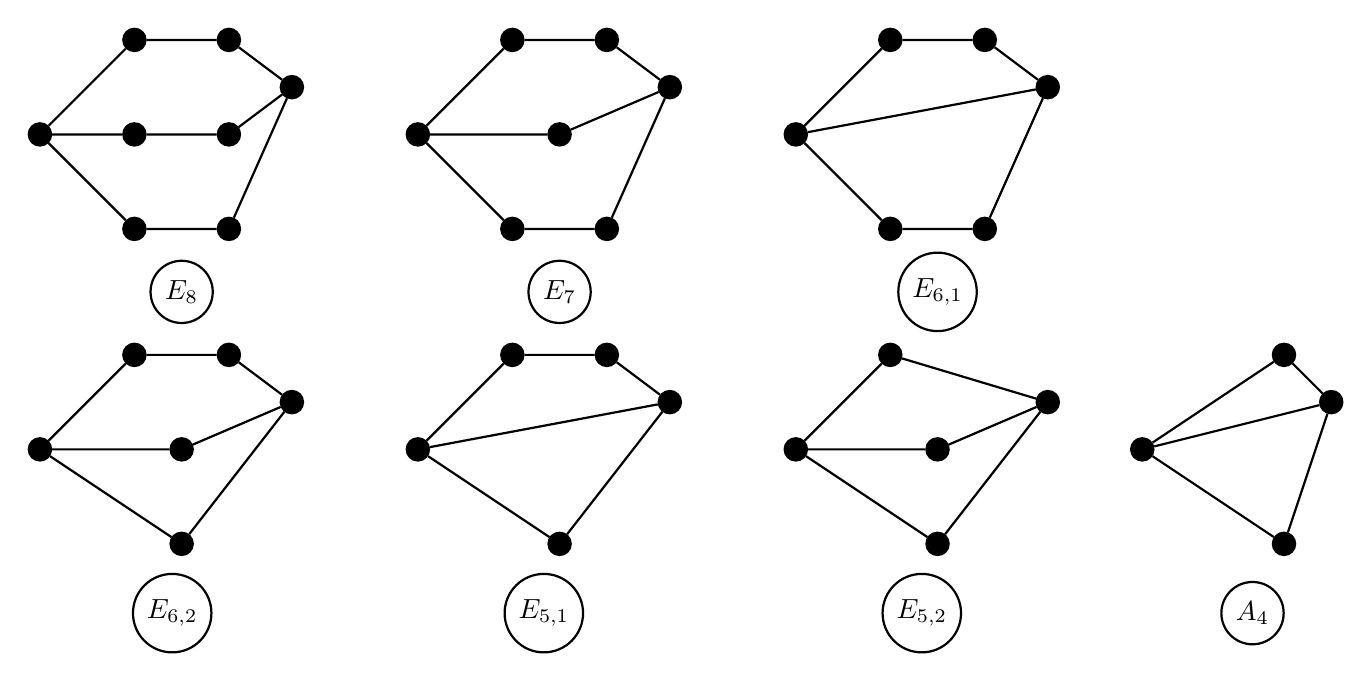
\begin{tikzpicture}
		[scale=0.4,inner sep=8mm, % this is the node radius
		vertex/.style={circle,thick,draw}, % this defines the default style for the vertex class
		thickedge/.style={line width=2pt}] % this defines the default style for the thick edges
		\node[vertex] (a1) at (0,0) [inner sep=1mm,fill=black] {};
		\node[vertex] (a2) at (3,3) [inner sep=1mm,fill=black] {};  
		\node[vertex] (a3) at (6,3) [inner sep=1mm,fill=black] {};   
		\node[vertex] (a4) at (8,1.5) [inner sep=1mm,fill=black] {};   
		\node[vertex] (a5) at (3,-3) [inner sep=1mm,fill=black] {};   
		\node[vertex] (a6) at (6,-3) [inner sep=1mm,fill=black] {};  
		\node[vertex] (a7) at (3,0) [inner sep=1mm,fill=black] {};   
		\node[vertex] (a8) at (6,0) [inner sep=1mm,fill=black] {};  
\draw[thick,black] (a1)--(a2) (a1)--(a5) (a1)--(a7) (a2)--(a3) (a3)--(a4) (a4)--(a6) (a4)--(a8) (a5)--(a6) (a7)--(a8);     
\node[vertex] (A) at (4.5,-5) [inner sep=1.mm,fill=white] {$E_8$};    
%%%%%%%%%%%%%%%%%
\node[vertex] (b1) at (12,0) [inner sep=1mm,fill=black] {};
		\node[vertex] (b2) at (15,3) [inner sep=1mm,fill=black] {};  
		\node[vertex] (b3) at (18,3) [inner sep=1mm,fill=black] {};   
		\node[vertex] (b4) at (20,1.5) [inner sep=1mm,fill=black] {};   
		\node[vertex] (b5) at (15,-3) [inner sep=1mm,fill=black] {};   
		\node[vertex] (b6) at (18,-3) [inner sep=1mm,fill=black] {};  
		\node[vertex] (b78) at (16.5,0) [inner sep=1mm,fill=black] {};   
\draw[thick,black] (b1)--(b2) (b1)--(b5) (b2)--(b3) (b3)--(b4) (b4)--(b6) (b5)--(b6) (b1)--(b78) (b78)--(b4); 
\node[vertex] (B) at (16.5,-5) [inner sep=1.mm,fill=white] {$E_7$};  
%%%%%%%%%%%%%%%%%%%%%%
%%%%%%%%%%%%%%%%%
\node[vertex] (c1) at (24,0) [inner sep=1mm,fill=black] {};
		\node[vertex] (c2) at (27,3) [inner sep=1mm,fill=black] {};  
		\node[vertex] (c3) at (30,3) [inner sep=1mm,fill=black] {};   
		\node[vertex] (c4) at (32,1.5) [inner sep=1mm,fill=black] {};   
		\node[vertex] (c5) at (27,-3) [inner sep=1mm,fill=black] {};   
		\node[vertex] (c6) at (30,-3) [inner sep=1mm,fill=black] {};     
\draw[thick,black] (c1)--(c2) (c1)--(c5) (c2)--(c3) (c3)--(c4) (c4)--(c6) (c5)--(c6) (c1)--(c4);  
\node[vertex] (C) at (28.5,-5) [inner sep=1.mm,fill=white] {$E_{6,1}$}; 
%%%%%%%%%%%%%%%%%%%
	\node[vertex] (d1) at (0,-10) [inner sep=1mm,fill=black] {};
		\node[vertex] (d2) at (3,-7) [inner sep=1mm,fill=black] {};  
		\node[vertex] (d3) at (6,-7) [inner sep=1mm,fill=black] {};   
		\node[vertex] (d4) at (8,-8.5) [inner sep=1mm,fill=black] {};   
		\node[vertex] (d56) at (4.5,-13) [inner sep=1mm,fill=black] {};   
		\node[vertex] (d78) at (4.5,-10) [inner sep=1mm,fill=black] {};   
\draw[thick,black] (d1)--(d2) (d1)--(d56) (d1)--(d78) (d2)--(d3) (d3)--(d4) (d4)--(d56) (d4)--(d78);   
\node[vertex] (D) at (4.2,-15.2) [inner sep=1.mm,fill=white] {$E_{6,2}$};  
%%%%%%%%%%%%%%%%%%%
	\node[vertex] (e1) at (12,-10) [inner sep=1mm,fill=black] {};
		\node[vertex] (e2) at (15,-7) [inner sep=1mm,fill=black] {};  
		\node[vertex] (e3) at (18,-7) [inner sep=1mm,fill=black] {};   
		\node[vertex] (e4) at (20,-8.5) [inner sep=1mm,fill=black] {};   
		\node[vertex] (e56) at (16.5,-13) [inner sep=1mm,fill=black] {};   
\draw[thick,black] (e1)--(e2) (e1)--(e4) (e1)--(e56) (e2)--(e3) (e3)--(e4) (e4)--(e56);
\node[vertex] (E) at (16,-15.2) [inner sep=1.mm,fill=white] {$E_{5,1}$}; 
%%%%%%%%%%%%%%%%%
%%%%%%%%%%%%%%%%%%
	\node[vertex] (f1) at (24,-10) [inner sep=1mm,fill=black] {};
		\node[vertex] (f23) at (27,-7) [inner sep=1mm,fill=black] {};     
		\node[vertex] (f4) at (32,-8.5) [inner sep=1mm,fill=black] {};   
		\node[vertex] (f56) at (28.5,-13) [inner sep=1mm,fill=black] {};   
		\node[vertex] (f78) at (28.5,-10) [inner sep=1mm,fill=black] {};   
\draw[thick,black] (f1)--(f23) (f1)--(f56) (f1)--(f78) (f23)--(f4) (f4)--(f56) (f4)--(f78); 
\node[vertex] (F) at (28.,-15.2) [inner sep=1.mm,fill=white] {$E_{5,2}$}; 
%%%%%%%%%%%%%%%%%%%    
%%%%%%%%%%%%%%%%%%%
	\node[vertex] (g1) at (35,-10) [inner sep=1mm,fill=black] {};
		\node[vertex] (g23) at (39.5,-7) [inner sep=1mm,fill=black] {};  
		\node[vertex] (g4) at (41,-8.5) [inner sep=1mm,fill=black] {};   
		\node[vertex] (g56) at (39.5,-13) [inner sep=1mm,fill=black] {};   
\draw[thick,black] (g1)--(g23) (g1)--(g4) (g1)--(g56) (g23)--(g4) (g4)--(g56);\node[vertex] (G) at (38.5,-15.2) [inner sep=1.mm,fill=white] {$A_{4}$}; 
%%%%%%%%%%%%%%%%%   
		\end{tikzpicture}
	\end{center}
	\caption{All graphs corresponding to $2\leq a \leq b \leq c \leq 4$ in $G_2^*$ of type~III.} \label{fig:2abc4}
	\end{figure}
	
\begin{align*}
&\N(A_4)=14 \,,~~ \N(A_4)_v \leq 8\,,\\
&\N(E_{5,2})=26 \,,~~ \N(E_{5,2})_v \leq 15\,,\\
&\N(E_{5,1})= 24\,,~~ \N(E_{5,1})_v \leq 14\,,\\
&\N(E_{6,2})= 42\,,~~ \N(E_{6,2})_v \leq 25\,,\\
&\N(E_{6,1})= 40\,,~~ \N(E_{6,1})_v \leq 25\,,\\
&\N(E_{7})=66 \,,~~ \N(E_{7})_v \leq 41\,,\\
&\N(E_{8})=100 \,,~~ \N(E_{8})_v \leq 64\,,
\end{align*}
where $v$ is any vertex in these graphs (the details are omitted). Recall that $n\geq 8$ and that $G_2 \in \mathbb{B}_n$ consists of
$$G_2^*\in \{A_4,E_{5,2}, E_{5,1}, E_{6,2}, E_{6,1}, E_{7}, E_{8}\}$$ and pendant edges, all of which are attached to the same vertex $v$ of $G_2^*$. With $m=|V(G_2^*)|$ and $u$ the center of $S_{n-m+1}$, we employ Lemma~\ref{Lem:identify} to obtain
\begin{align*}
\N(G_2)&=\N(G_2^*)+\N(S_{n-m+1}) -1 + (\N(G_2^*)_v-1)(\N(S_{n-m+1})_u - 1)\\
&=\N(G_2^*)+ (2^{n-m}+n-m) -1 + (\N(G_2^*)_v-1)(2^{n-m}- 1)\,.
\end{align*}
Hence, the following hold:
\begin{align*}
\N(G_2) \leq ~~& 26 + (2^{n-5}+n-5) -1 + (15 -1)(2^{n-5}- 1)=15 \cdot 2^{n-5}+6+n\\
&= 2^{n-1} -2^{n-5}+6+n < 2^{n-1} +1+n = \N(R_n)
\end{align*}
for $G_2^* \in \{E_{5,2},E_{5,1}\}$, and
\begin{align*}
\N(G_2)  \leq & ~~ 42 + (2^{n-6}+n-6) -1 + (25 -1)(2^{n-6}- 1)=25 \cdot 2^{n-6}+11+n\\
&= 2^{n-1} -7 \cdot 2^{n-6}+11+n < 2^{n-1} +1+n = \N(R_n)
\end{align*}
for $G_2^* \in \{E_{6,2},E_{6,1}\}$, and
\begin{align*}
\N(G_2)  \leq & ~~ 66 + (2^{n-7}+n-7) -1 + (41 -1)(2^{n-7}- 1)=41 \cdot 2^{n-7}+18+n\\
&= 2^{n-1} -23 \cdot 2^{n-7}+18+n < 2^{n-1} +1+n = \N(R_n)
\end{align*}
for $G_2^* =E_7$, and
\begin{align*}
\N(G_2)  \leq & ~~ 100 + (2^{n-8}+n-8) -1 + (64 -1)(2^{n-8}- 1)=64 \cdot 2^{n-8}+28+n\\
&= 2^{n-1} -64 \cdot 2^{n-8}+28+n < 2^{n-1} +1+n = \N(R_n)
\end{align*}
for $G_2^* =E_8$. In all these cases, we get $\N(G_2) < \N(R_n) =\N(B_n)-1 < \N(B_n)$. Since the case where $G_2^* =A_4$ defines the graph $B_n$, we are done with he proof of the theorem.
\end{itemize}
In particular, $R_n$ is the second-largest $n$-vertex bicyclic graph with respect to the number of connected sets.
\end{proof}


\medskip
\section*{Statements and Declarations}

The author did not receive support from any organization for the submitted work. The author has no competing interests to declare that are relevant to the content of this article.

\medskip

\begin{thebibliography}{10}

\bibitem{Nordhauss}	
E.~O.~D.~Andriantiana, A.~A.~V.~Dossou-Olory.
\newblock Nordhaus-Gaddum inequalities for the number of connected induced subgraphs in graphs.
\newblock {\em Quaest. Math.}, 45(8) 1191--1213, 2022.
    
\bibitem{Audacegenral2018}
A.~A.~V.~Dossou-Olory.
\newblock Graphs and unicyclic graphs with extremal number of connected subgraphs.
\newblock {\em Indian J. Discrete Math.}, 8 (2) 47--67, 2022.
    
\bibitem{AudaceGirth2018}
A.~A.~V.~Dossou-Olory.
\newblock Maximising the number of connected induced subgraphs of unicyclic graphs.
\newblock {\em Turk. J. Math.}: 46(8), Art. 19, 3359--3372, 2022.
	
\bibitem{AudaceCut2019}
A.~A.~V.~Dossou-Olory.
\newblock Cut and pendant vertices and the number of connected induced subgraphs of a graph.
\newblock {\em Eur. J. Math.} 7:766--792, 2021. 

%\bibitem{AudaceTOUT}
%A.~A.~V.~Dossou-Olory.
%\newblock Cut and pendant vertices and the number of connected induced subgraphs of a graph.
%\newblock {\em Eur. J. Math.} 7:766--792, 2021. 

\bibitem{AudTOUT}
A.~A.~V.~Dossou-Olory.
\newblock Cut vertex and unicyclic graphs with the maximum number of connected induced subgraphs.
\newblock {\em J. Combin. Math. Combin. Comput.} 128:119--142, 2026. 
	
%%%%%%%%%%%%%%%%%%%%%%%%


\bibitem{AndriantianaV2021}
E.~O.~D.~Andriantiana, V.~R.~Misanantenaina, and S.~Wagner.
\newblock Extremal trees with fixed degree sequence.
\newblock {\em Electr. J. Combin.} 28(1), \# P1.1., 2021.

\bibitem{Andriantiana2017}
E.~O.~D.~Andriantiana, S.~Wagner, and H.~Wang.
\newblock Extremal problems for trees with given segment sequence.
\newblock {\em Discr. Appl. Math.} 220, 20--34, 2017.

\bibitem{Andriantiana2013}
E.~O.~D.~Andriantiana, S.~Wagner, and H.~Wang.
\newblock Greedy trees, subtrees and antichains.
\newblock {\em Electronic J. Combin.} 20(3) \# P28, 2013.

\bibitem{ZichongChen}
Z.~Chen.
\newblock The number of subtrees of trees with given diameter.
\newblock {\em Discr. Math. Alg. Appl.} 10(01), \# 1850001, 2018.

\bibitem{AudDank2020}
P.~Dankelmann, A.~A.~V.~Dossou-Olory.
\newblock Wiener index, number of subtrees, and tree eccentric sequence.
\newblock {\em MATCH Commun. Math. Comput. Chem.} 84:611--628, 2020.

\bibitem{Milo2002}
R.~Milo, S. ~hen-Orr, S.~Itzkovitz, N.~Kashtan, D.~Chklovskii, and U.~Alon. 
\newblock Network motifs: simple building blocks of complex networks. 
\newblock {\em Science} 298(5594):824--827, 2002.


\bibitem{Wang2005}
L.~A.~Sz\'ekely, H.~Wang.
\newblock On subtrees of trees.
\newblock {\em Adv. Appl. Math.} 34:138--155, 2005.

\bibitem{Wang2005Plus}
L.~A.~Sz\'ekely, H.~Wang.
\newblock Binary trees with the largest number of subtrees with at least one leaf. 
\newblock {\em Congr. Numer.} 177:147--169, 2005.
%%%%%%%%%%%%%
%\bibitem{Yuzhi2017}
%Y.~Xiao, H.~Zhao, Z.~Liu, and Y.~Mao.
%\newblock Trees with large numbers of subtrees.
%\newblock {\em International J. Computer Math.} 94:2, 372--385, 2017.
%	
\bibitem{Zhang2015}
X.-M.~Zhang, X.-D.~Zhang.
\newblock The minimal number of subtrees with a given degree sequence.
\newblock {\em Graphs Combin.} 31:309--318, 2015.

\bibitem{ZhangZhang2013}
X.-M.~Zhang, X.-D.~Zhang, D.~Gray, and H.~Wang.
\newblock The number of subtrees of trees with given degree sequence.
\newblock {\em J. Graph Theory} 73(3):280--295, 2013.



\end{thebibliography}


\end{document}
